\documentclass[10pt]{beamer}

\usefonttheme{professionalfonts} % using non standard fonts for beamer
\usefonttheme{serif} % default family is serif
\usepackage{amsmath}
\usepackage{ulem}
\usepackage{hyperref}
\usepackage{array}
\usepackage{mathtools}
\usepackage{epsf}
\geometry{paperwidth=160mm,paperheight=120mm}
\def\LL{\left\langle}	% left angle bracket
\def\RR{\right\rangle}	% right angle bracket
\def\LP{\left(}		% left parenthesis
\def\RP{\right)}	% right parenthesis
\def\LB{\left\{}	% left curly bracket
\def\RB{\right\}}	% right curly bracket
\def\PAR#1#2{ {{\partial #1}\over{\partial #2}} }
\def\PARTWO#1#2{ {{\partial^2 #1}\over{\partial #2}^2} }
\def\PARTWOMIX#1#2#3{ {{\partial^2 #1}\over{\partial #2 \partial #3}} }

\def\BI{\begin{itemize}}
\def\EI{\end{itemize}}
\def\BAL{\begin{align*}}
\def\EAL{\end{align*}}
\def\BS{\bigskip}
\def\BC{\begin{center}}
\def\EC{\end{center}}
\def\BCC{\begin{columns}}
\def\ECC{\end{columns}}
\def\HC{\column{0.5\textwidth}}

\newcommand{\etal}{{\it et al.}}
\newcommand{\ie}{{\em i.e.\ }}
\newcommand{\eg}{{\em e.\,g.\ }}
\newcommand{\etc}{etc.\ }
\newcommand{\dt}{\Delta t}

%AB: my color definitions
\definecolor{abtitlecolor}{rgb}{0.0,0.255,0.494}
\definecolor{absecondarycolor}{rgb}{0.0,0.416,0.804}
\definecolor{abprimarycolor}{rgb}{1.0,0.686,0.0}
\definecolor{Red}           {cmyk}{0,1,1,0}
\definecolor{Grey}           {cmyk}{.7,.7,.7,0}
\definecolor{Lg}           {cmyk}{.4,.4,.4,0}
\definecolor{Blue}          {cmyk}{1,1,0,0}
\definecolor{Green}         {cmyk}{1,0,1,0}
\definecolor{Brown}         {cmyk}{0,0.81,1,0.60}
\definecolor{Black}         {cmyk}{0,0,0,1}
\definecolor{A}{rgb}{0.8,0.0,0.0}
\definecolor{B}{rgb}{0.0,0.6,0.0}
\definecolor{C}{rgb}{0.6,0.6,0.0}
\definecolor{D}{rgb}{0.0,0.0,0.5}
\definecolor{E}{rgb}{0.4,0.4,0.4}

\usetheme{Madrid}

%AB: redefinition of beamer colors
\setbeamercolor{title}{fg=abtitlecolor}
\setbeamercolor{frametitle}{fg=abtitlecolor}
\setbeamercolor{palette tertiary}{fg=white,bg=abtitlecolor}
\setbeamercolor{palette secondary}{fg=white,bg=absecondarycolor}
\setbeamercolor{palette primary}{fg=black,bg=abprimarycolor}
\setbeamercolor{structure}{fg=abtitlecolor}

\setbeamerfont{section in toc}{series=\bfseries}

%AB: remove navigation icons
\beamertemplatenavigationsymbolsempty


\title{
  \textbf {Introduction to kinematics}\\
}

\author[W. Freeman] {Physics 211\\Syracuse University, Physics 211 Spring 2019\\Walter Freeman}

\date{\today}

\begin{document}

\frame{
\large
\begin{center}
My purpose is to set forth a very new science dealing with a very ancient subject.
There is, in nature, perhaps nothing older than motion,
concerning which the books written by philosophers are neither few nor small
nevertheless I have discovered by experiment some properties of it which are worth
knowing and which have not hitherto been either observed or demonstrated....

\bigskip

So far as I know, no one has yet pointed out that the distances traversed, during equal intervals of time, by a body falling from rest,
stand to one another {\bf in the same ratio as the odd numbers beginning with unity.}
\bigskip
\end{center}
\bigskip
\begin{flushright}
\normalsize
--Galileo Galilei, {\it Dialogues and Mathematical Demonstrations Concerning Two New Sciences}, 1638
\end{flushright}
}



\frame{\titlepage}

\frame{\frametitle{\textbf{Reminders:}}
\Large
\begin{itemize}
\item Webpage: {https://walterfreeman.github.io/phy211/}
\BI
\large
\item Syllabus, homework, etc. are all there
\EI
\item The first homework is due next Friday
\item Please fill out the survey linked from the first page by the end of the day tomorrow
\EI
}

\frame{\frametitle{\textbf{Using Slack}}
Slack is basically Discord for professionals. It's a more efficient way than email for you all to ask for help
and discuss our class.

\BS

There's a link on the course website to join (and clients for Linux, Windows, macOS, iThings, Android...)

\BS\BS

Please make sure you use the different channels for what they're designed for:

\BI
\item Memes and so forth go in \#random
\item Discussions of homework go in \#homework1, \#homework2, etc.
\item To join a channel (like a Discord room), you can type ``/join \#homework1'' or click on ``channels'' on the left
\item If you have a question that other people may care about too, post it in a public channel and tag me (@Walter Freeman), rather than PM'ing me
\EI

\BS\pause

Please be decent to each other: I already had to banhammer someone for making an account impersonating an instructor (if that was you, just make another account). 
}


\frame{\frametitle{\textbf{``Ask a Physicist''}}
\BC
\large There are a lot of cool things in physics that go beyond mechanics.
\EC
\bigskip
\bigskip

\normalsize

If you've got questions you'd like me to address, send them in and I'll answer them!
(Good questions may earn you extra credit!)

\BI
\item What are gravity waves?
\item Is there life on other planets?
\item Is Pluto a planet?
\item{What's the Large Hadron Collider for?}
\item{What is quantum gravity?}
\item{How do 3D movies work?}
\item{What is the Higgs boson?}
\item{How is physics used in video games?}
\item{How does a nuclear bomb work?}
\item{Could we travel through wormholes?}
\EI
}

\frame{\frametitle{\textbf{Homework tips}}
\centerline{\large Your first homework assignment is due next Friday.}

\bigskip
\bigskip

\BI
\item{Make use of words, pictures, and algebra (not {\it just} algebra!) in your reasoning}
\item{We're interested in how you think, not just the answer.}
\item{Physical values need to be given with units (``4 meters'', not ``4'')}
\item{Leave variables in until the very end}
\item{Paper is cheap -- use an entire side of paper for each problem.}
\pause
\bigskip
\item{Ask for help -- early and often}
\BI
\item{Email: wafreema@g.syr.edu}
\item{Slack channel (better than email)}
\item{Office hours}
\item{The Physics Clinic -- room 112}
\item{Recitations}
\pause
\item{In class!}
\EI
\EI
}

\frame{\frametitle{\textbf{The course webpage}}
\large
\BI
\item{All notes, etc., will be posted on the course website (not Blackboard)}
\item{I will also post course announcements there (and as stickied posts in \#general on Slack)}
\item{The syllabus is posted there}
\item{You really should read the section on the course philosophy}
\EI
}

\frame{\frametitle{\textbf{Office hours}}
\Large
In the Physics Clinic (room 112):
\BI
\item This Friday: 9:30-11:30 AM
\item Other times announced (to help you best with homework) 
\item {\bf Next week: Wednesday 2-6 PM and Thursday 1:45-3:45 PM, focusing on Homework 1}
\EI
\BS
or by appointment.
\bigskip
\bigskip

Outside these times you might find me in the Clinic or in my office in room 215.
}


\frame{\frametitle{\textbf{The beginning: Free fall}}
\centerline{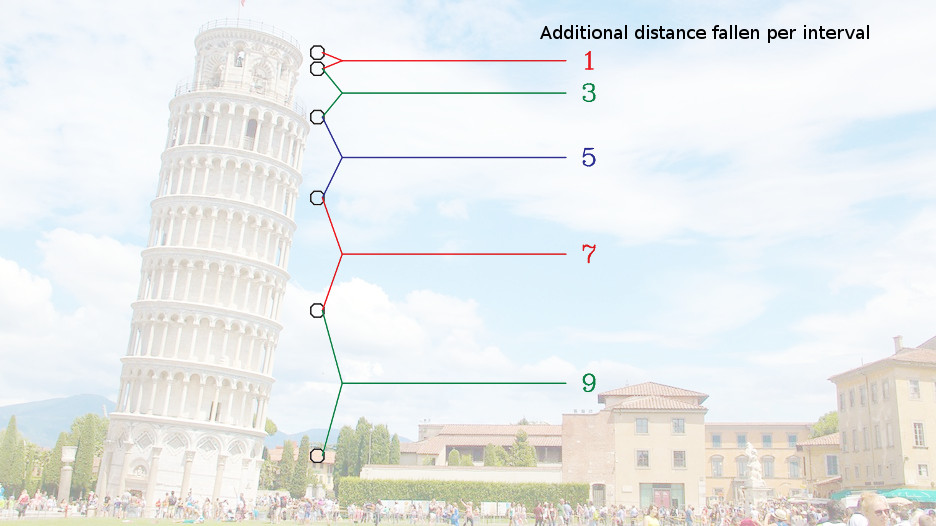
\includegraphics[width=0.9\textwidth]{pisa.jpg}}

\begin{center}
\Large Galileo observed this, but can we explain it?
\end{center}
}



\frame{\frametitle{\textbf{Equations of motion}}
Complete description of motion: ``Where is my object at each point in time?''

\bigskip

This corresponds to a mathematical function. Two ways to represent these. Suppose I drop
a ball off a building, putting the origin at the ground and calling ``up'' the positive direction:

\bigskip
\bigskip

\begin{columns}
\column{0.5\textwidth}
\centerline {\color{Red}\Large Graphical representation}
\column{0.5\textwidth}
\centerline{\color{Blue} \Large Algebraic representation}
\end{columns}

\bigskip

\begin{columns}
\column{0.5\textwidth}

\centerline{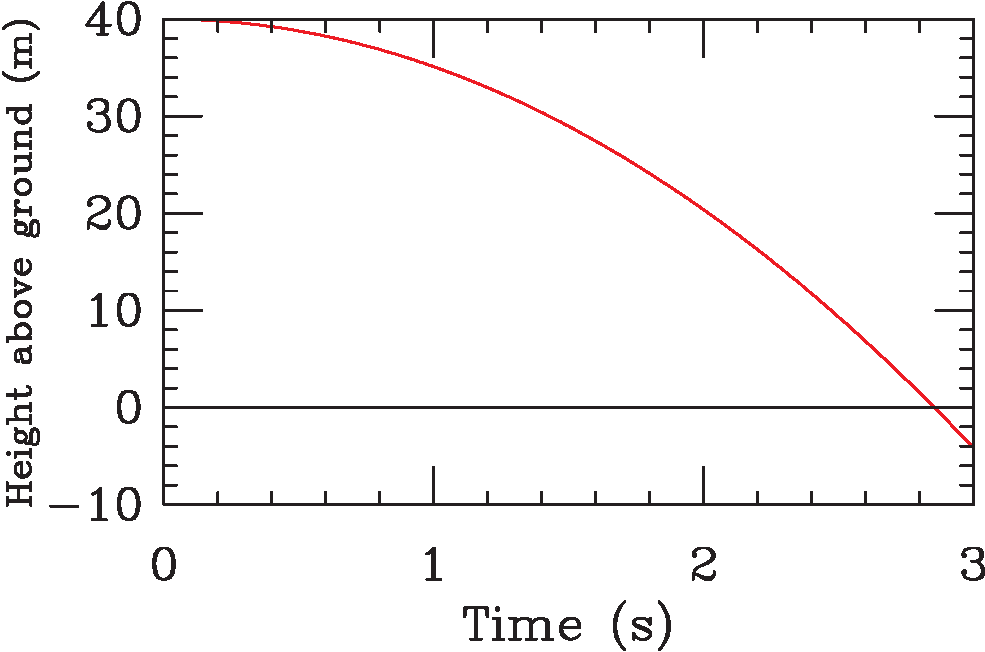
\includegraphics[width=0.7\textwidth]{falling-crop.pdf}}

\column{0.5\textwidth}
\color{Blue}
$$y(t) = (40 \,{\mathrm m}) - C t^2$$ \\
(C is some number)

\end{columns}

\bigskip

\centerline{Both let us answer questions like ``When does the object hit the ground?''}

\bigskip

\begin{columns}
\column{0.5\textwidth}
\centerline {\color{Red}\large $\rightarrow$ ... the curve's x-intercept}
\column{0.5\textwidth}
\centerline{\color{Blue} \large $\rightarrow$ ... when $y(t)=0$}
\end{columns}

}

\frame{\frametitle{\textbf{Velocity: how fast position changes}}
The slope of the position vs. time curve has a special significance. Here's one with a constant slope:

\medskip

\centerline{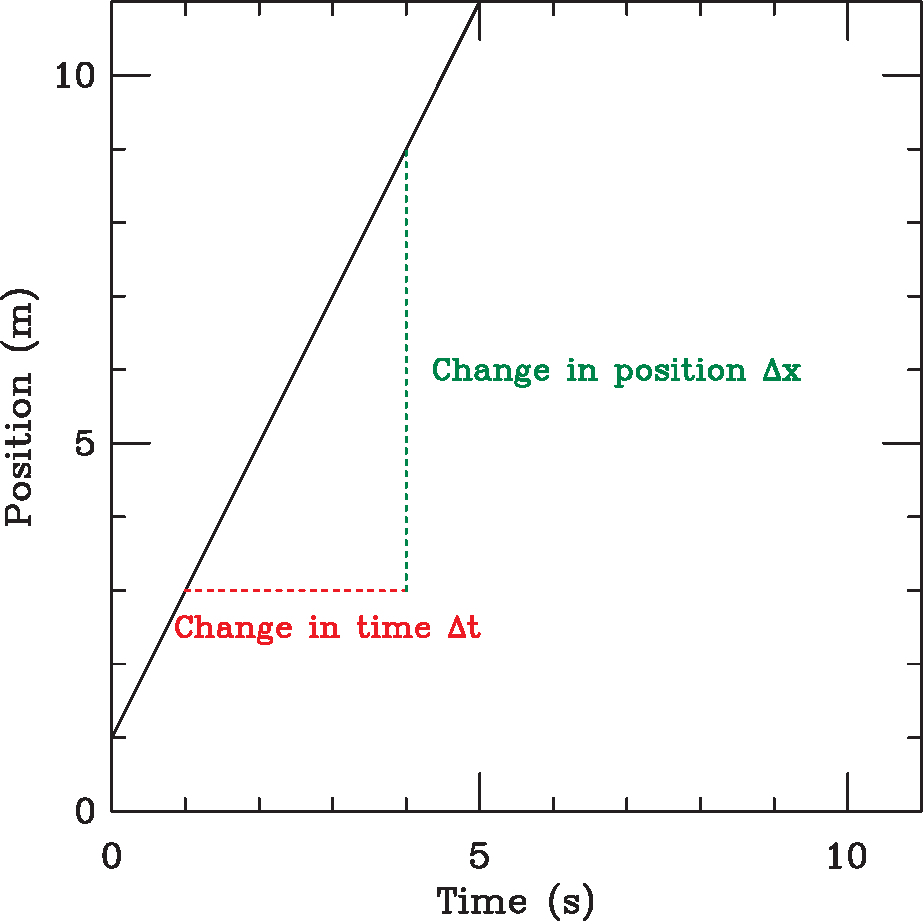
\includegraphics[width=0.4\textwidth]{constant-v-crop.pdf}}

\bigskip

\pause

Slope is $\frac{{\rm rise}}{{\rm run}}$ = $\frac{\Delta x}{\Delta t}$ = $\frac{2\,\rm m}{1 \, \rm s}$ = 2 meters per second (positive;
it could well be negative!)

\bigskip \pause

{\color{Red} $\rightarrow$ The slope here -- change in position over change in time -- is the {\bf velocity}!} \\Note that it can be
positive or negative, depending on which way the object moves.

}


\frame{\frametitle{\textbf{Constant-$v$ motion: connecting graphs to algebra}}
If an object moves with constant velocity, its position vs. time graph is a line:

\medskip

\centerline{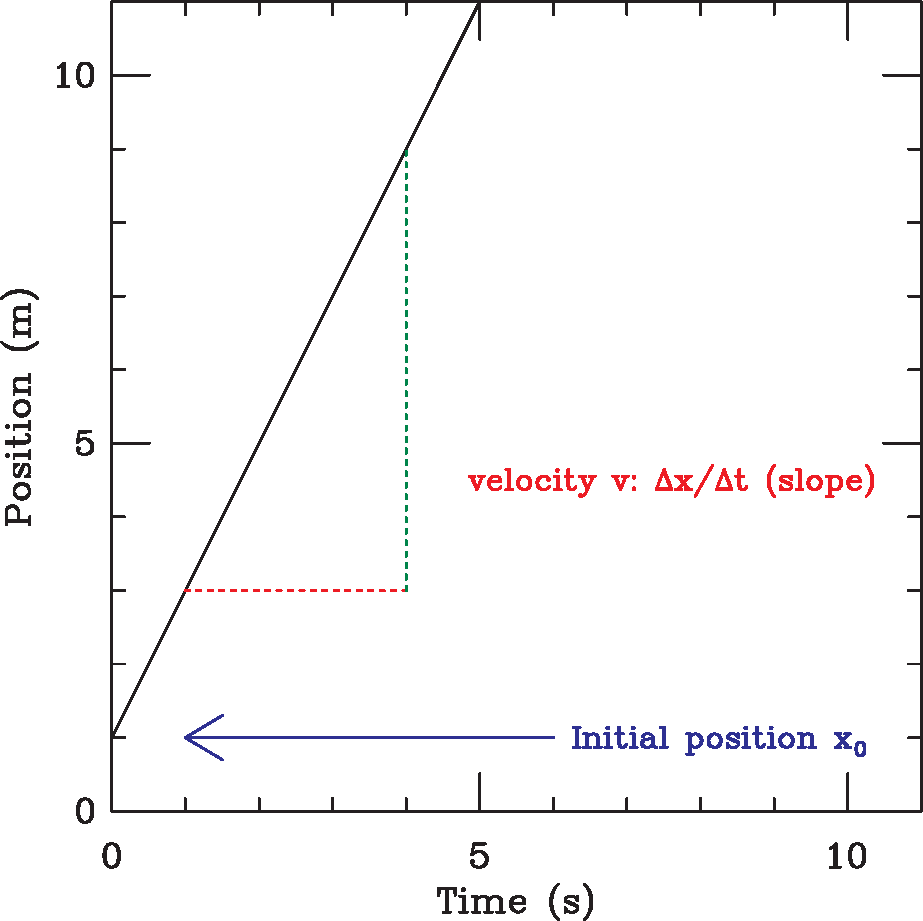
\includegraphics[width=0.4\textwidth]{constant-v-2-crop.pdf}}

We know the equation of a straight line is is $x = mt + b$ (using $t$ and $x$ as our axes).

\BI
\item{$m$ is the slope, which we identified as the velocity}
\item{$b$ is the vertical intercept, which we recognize as the value of $x$ when $t=0$}
\EI

We can thus change the variable names to be more descriptive:

\bigskip

\centerline{\Large{{\color{Red} $x(t) = vt + x_0$} (constant-velocity motion)}}

}

\frame{\frametitle{\textbf{Going from ``equations of motion'' to answers}}

\large

{\color{Red}$x(t) = vt + x_0$} is called an {\it equation of motion}; in this case, it is valid for constant-velocity motion.

\medskip

It gives you the same information as a position vs. time graph, but in algebraic form.

\bigskip
\bigskip

\normalsize

To solve real problems, we need to be able to translate physical questions into algebraic statements:
\bigskip
\bigskip

\BI
\item{``If a car starts at milepost 30 and drives at 50 mph, where is it an hour later?''}
\pause
\BI
\item{Using $x(t) = x_0 + vt$, with $x_0=30\, {\rm mi}$ and $v = 50 \frac{\rm mi}{\rm hr}$, calculate $x$ at $t=1\, {\rm hr}$}
\EI
\EI
}

\frame{\frametitle{\textbf{Asking the right questions}}
\large
``I drop an object from a height $h$. When does it hit the ground?'' How do I
do this? (Take $x_0=h$ and upward to be positive.)

\BS
\large
Remember, we want to ask a question in terms of our physical variables. This question 
has the form:

\BS
\Large
``What is \rule{1in}{0.55mm} at the time that \rule{1in}{0.55mm} equals \rule{1in}{0.55mm}?''

\BS
\BC
\large
Fill in the blanks.

\Large
\BS

\color{A}A: $v$, $x$, 0 \\
\color{B}B: $t$, $x$, h \\
\color{C}C: $x$, $t$, 0 \\
\color{D}D: $t$, $x$, 0 \\
\color{E}E: $x$, $v$, 0 \\
\EC
}

\frame{\frametitle{\textbf{Asking the right questions}}
\BC \Large ``At what location do two moving objects meet?''\EC

\BS
\Large
\color{A}A: ``At what time does $x_1 = x_2$?'' \\
\color{B}B: ``At what time does $v_1 = v_2$?'' \\
\color{C}C: ``What is $x_1$ at the time when $x_1 = x_2$?'' \\
\color{D}D: ``What is $x_1$ when $t_1 = t_2$?'' \\

\pause
\BS\BS
\large
\BC\color{Black}Writing sentences like these gives you a recipe for doing the algebra:\EC
\begin{enumerate}
\item Write down $x_1(t)$ and $x_2(t)$
\item Set these expressions equal and solve for the value of $t$ that makes that happen
\item Put that value of $t$ back into $x_1(t)$ or $x_2(t)$ to answer your question!
\end{enumerate}

}


\frame{\frametitle{\textbf{Velocity, acceleration, and calculus}}
\Large
Constant-velocity motion: $x(t) = x_0 + vt$

\normalsize

\BI

\item{Came from looking at the equation of a line}
\item{We can understand this in a different framework, too:}

\bigskip

\item{\Large Velocity is the {\color{Red} rate of change} of position}
\BI
\large
\item{Graphical representation: Velocity is the slope of the position vs. time graph}
\item{Mathematical language: Velocity is the {\color{Red} derivative} of position}
\EI
\EI

\bigskip
\bigskip

\Large

We know we need to know about acceleration (``F=ma'') -- what is it?

\bigskip
\BI
\item{Acceleration is the {\color{Red} rate of change} of velocity}
\EI
}


\frame{\frametitle{\textbf{Position, velocity, and acceleration}}
\begin{columns}
\column{0.125\textwidth}
\centerline{\Large Position}
\column{0.2\textwidth}
\footnotesize
{\color{Red}
\centerline{(take the derivative)}
\centerline{take the rate of change of}
\centerline{$\xrightarrow{\makebox[\textwidth]{}}$}}
\column{0.125\textwidth}
\centerline{\Large Velocity}
\pause
\column{0.2\textwidth}
\footnotesize
{\color{Red}
\centerline{(take the derivative)}
\centerline{take the rate of change of}
\centerline{$\xrightarrow{\makebox[\textwidth]{}}$}}
\column{0.15\textwidth}
\centerline{\Large Acceleration}
\end{columns}
}

\frame{\frametitle{\textbf{Kinematics: how does acceleration affect movement?}}
\large
Newton's law ${\color{A}a} = {\color{B}F}/{\color{C}m}$ tells us that {\it acceleration} -- the second derivative of position -- is what results from forces. 

\BS\large

All objects on Earth experience a downward force from Earth's gravity:

\BC {\color{B} (Force from gravity)} = {\color{C} (mass of object)} $\times$ {\color{D}(strength of Earth's gravity)} \EC

In symbols:

$${\color{B}F_g} = \color{C} m\color{D}g$$

Substituting this force into Newton's second law we get:

$${\color{A}a} = {\color{B}F_g} / {\color{C}m} = \color{C} m\color{D}g / \color{C} m$$

\bigskip\pause
\BC
This tells us that {\color{Red}all freely falling objects have a constant acceleration downward.}

The value of $g$ near Earth's surface is about $9.8 \mss$.

\EC
}

\frame{\frametitle{\textbf{All the calculus you need to know}}
\begin{center}
If velocity is the rate of change of position, \\
why is the area under the $v$ vs. $t$ curve equal to displacement?
\end{center}

\centerline{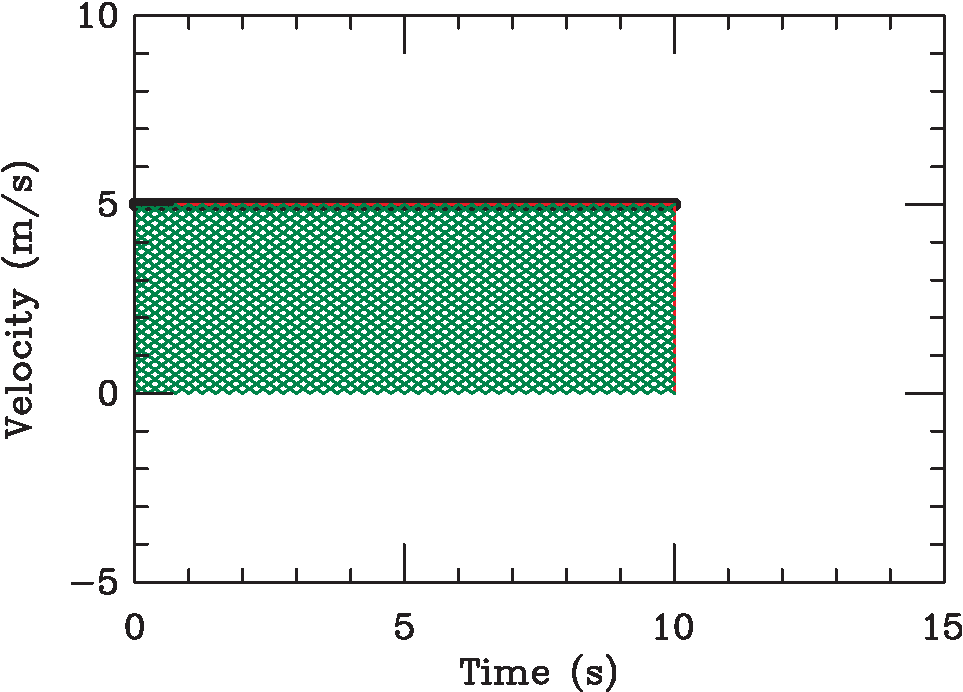
\includegraphics[width=0.7\textwidth]{integral-constant-crop.pdf}}

\bigskip
\bigskip

\centerline{We know $\Delta s = vt$. What is that here? What's the area of the shaded region?}

}

\frame{\frametitle{\textbf{A calculus review}}

\centerline{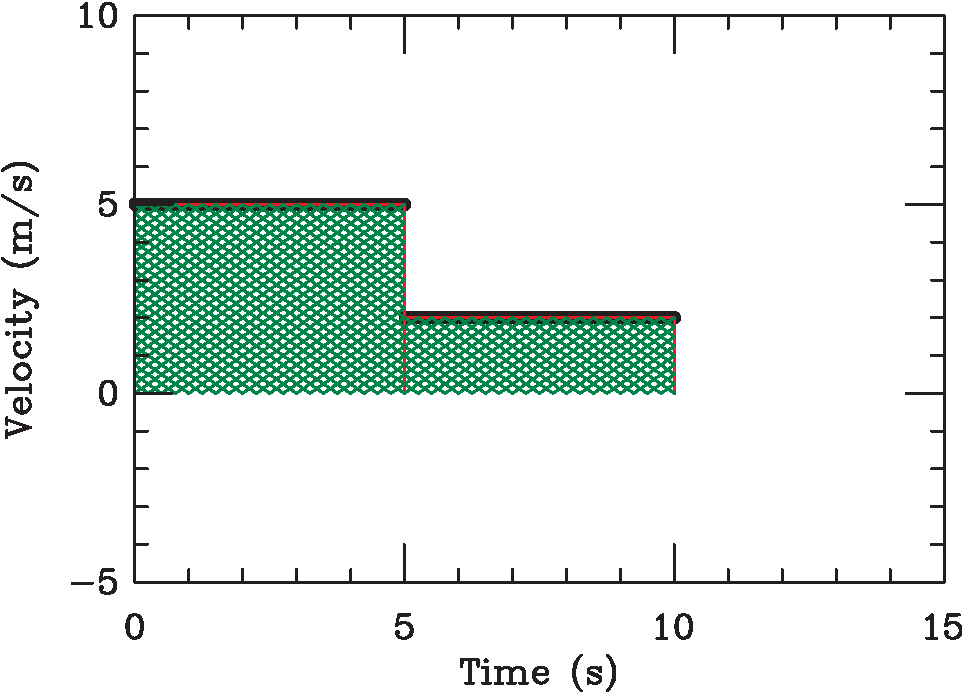
\includegraphics[width=0.6\textwidth]{integral-two-crop.pdf}}

\bigskip
\bigskip
\bigskip

\centerline{\large Now what is $\Delta s$? What is the area of the shaded region?}

}


\frame{\frametitle{\textbf{A calculus review}}

\centerline{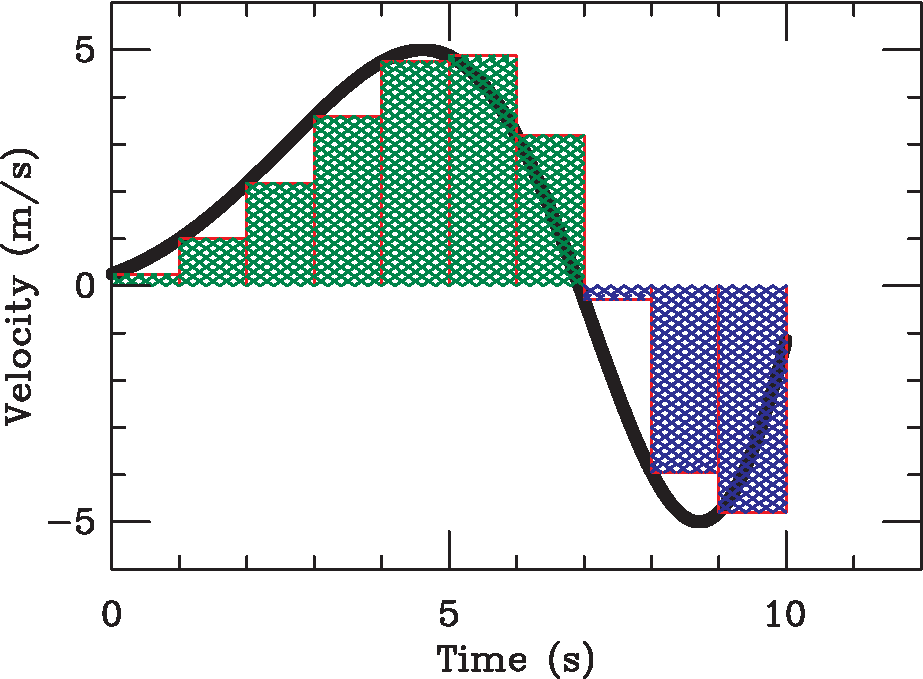
\includegraphics[width=0.6\textwidth]{integral-curve-coarse-crop.pdf}}

\bigskip
\bigskip
\bigskip

\centerline{\Large Does this work? How do we fix it?}

}
\frame{\frametitle{\textbf{A calculus review}}

\centerline{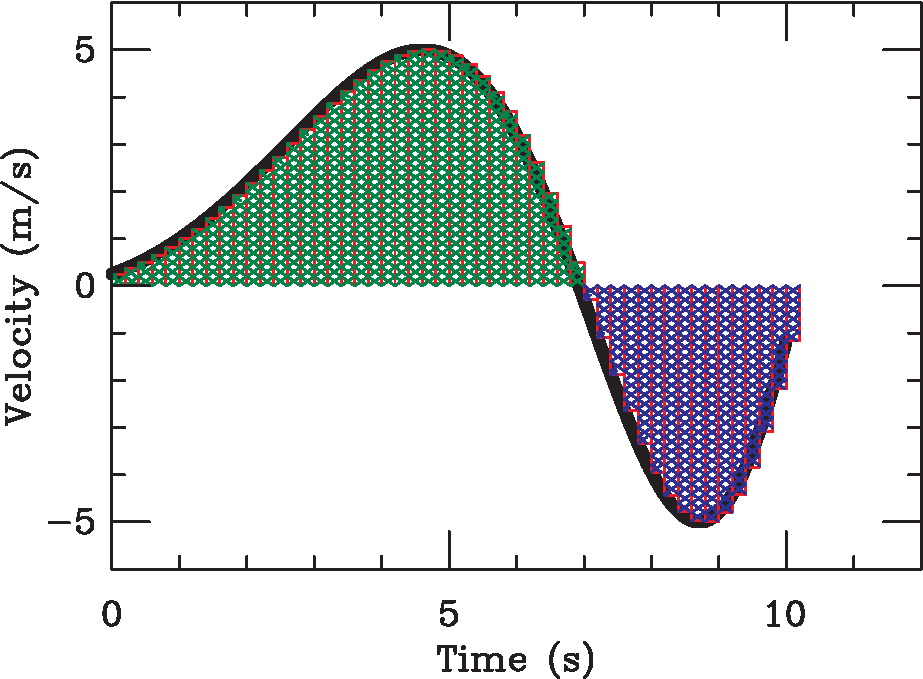
\includegraphics[width=0.6\textwidth]{integral-curve-fine-crop.pdf}}

\bigskip
\bigskip

\centerline{The area between the $t$-axis and the velocity curve is the distance traveled.}
\centerline{\color{Grey} (The area below the $t$-axis counts negative: ``the thing is going backwards''}
\bigskip
\centerline{In calculus notation: $\int v(t)\, dt = \delta x = x(t) - x_0$}

}

\frame{\frametitle{\textbf{Position, velocity, and acceleration}}
\begin{columns}
\column{0.125\textwidth}
\centerline{\Large Position}
\column{0.2\textwidth}
\footnotesize
{\color{Red}
\centerline{(take the derivative of)}
\centerline{take the rate of change of}
\centerline{$\xrightarrow{\makebox[\textwidth]{}}$}}
{\color{Green}
\color{Green}\centerline{$\xleftarrow{\makebox[\textwidth]{}}$}}
\color{Green}\centerline{take the area under the curve of}
\color{Green}\centerline{(take the integral of)}
\column{0.125\textwidth}
\centerline{\Large Velocity}
\pause
\column{0.2\textwidth}
\footnotesize
{\color{Red}
\centerline{(derivative of)}
\centerline{rate of change of}
\centerline{$\xrightarrow{\makebox[\textwidth]{}}$}}
{\color{Green}
\color{Green}\centerline{$\xleftarrow{\makebox[\textwidth]{}}$}}
\color{Green}\centerline{take the area under the curve of}
\color{Green}\centerline{(take the integral of)}
\column{0.15\textwidth}
\centerline{\large Acceleration}
\end{columns}
}

\frame{\frametitle{\textbf{Constant acceleration}}
Particularly interesting situation:
\BI
\item{Free fall (as you saw)}
\item{Any time the force is constant: $F = ma \rightarrow a = F/m$...}
\EI
\bigskip
\pause
Plan of attack:
\BI
\item{We know what the acceleration curve looks like (it's just flat)}
\item{Figure out the area under the acceleration curve to get the velocity curve}
\item{Figure out the area under the velocity curve to get the position curve}
\EI
\pause
\bigskip
\bigskip
\bigskip
\bigskip
Remember the area under the curve of (velocity, acceleration) just gives the {\it change in} (position, velocity) -- \ie initial minus final.

\bigskip
\bigskip

We'll start by assuming $x_0$ and $v_0$ are zero.
}

\frame{\frametitle{\textbf{Constant acceleration}}
\centerline{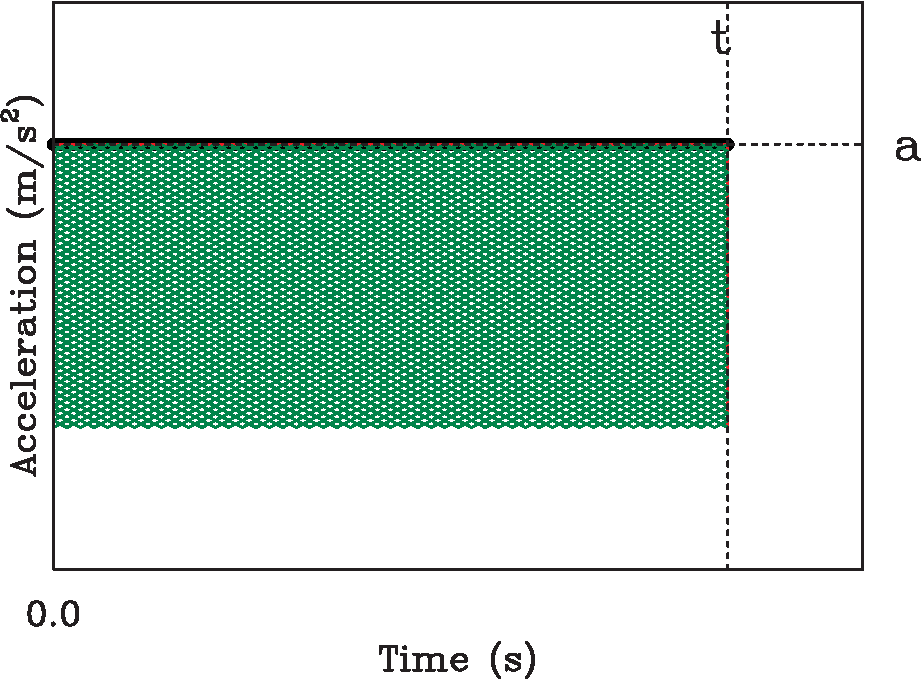
\includegraphics[width=0.6\textwidth]{area-under-a-crop.pdf}}

\bigskip

What's the area under the curve out to time $t$, which gives the change in the velocity -- $\Delta v=v(t) - v_0$?

\BS
\large
\BCC
\HC
\color{A}A: $\Delta v = at$\\
\color{C}C: $\Delta v = \frac{1}{2}at^2$\\
\HC
\color{B}B: $\Delta v = at + v_0$\\
\color{D}D: $\Delta v = a$\\
\ECC

}


\frame{\frametitle{\textbf{Constant acceleration}}
\centerline{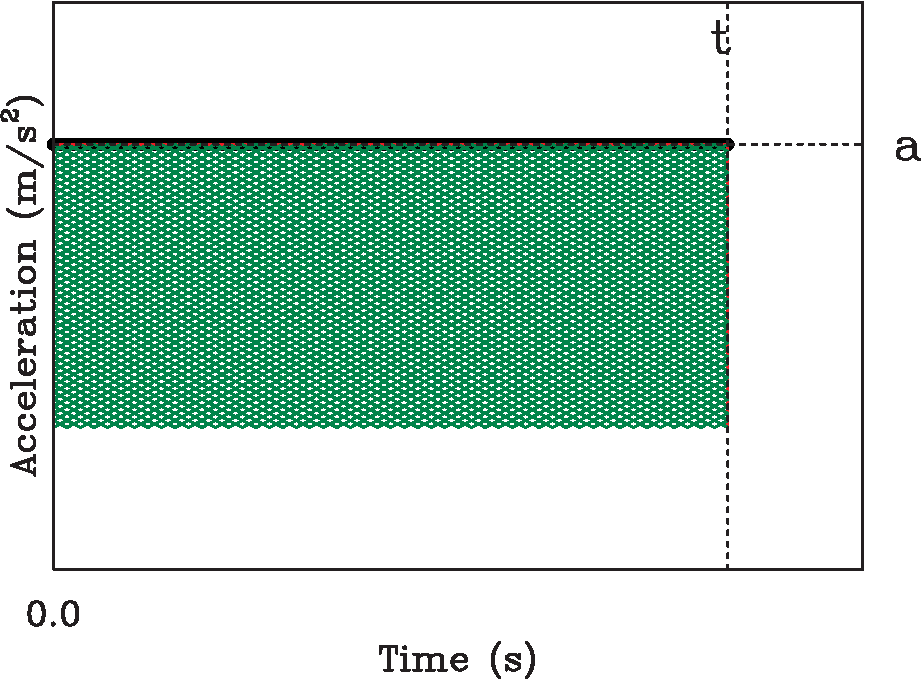
\includegraphics[width=0.6\textwidth]{area-under-a-crop.pdf}}

\bigskip

What's the area under the curve out to time $t$, which gives the change in the velocity -- $\Delta v=v(t) - v_0$?

\pause

\bigskip

\centerline{\large $\Delta v$, the change in velocity, is $v(t) - v_0 = at$, so {\color{Red}$v(t) = at + v_0$}}
}

\frame{\frametitle{\textbf{Do the same thing again to get position}}
\centerline{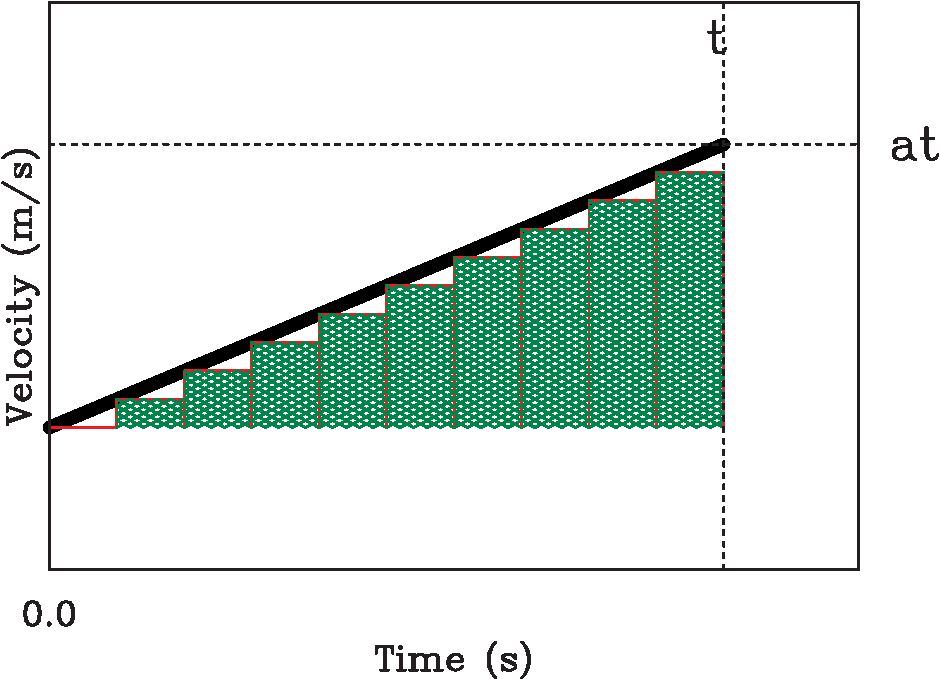
\includegraphics[width=0.6\textwidth]{area-under-v-crop.pdf}}

\bigskip

Now the area under the velocity curve gives the change in position: $\Delta x=x(t) - x_0$.
What is that?
\BS
\large
\BCC
\HC
\color{A}A: $\Delta x = at$\\
\color{C}C: $\Delta x = \frac{1}{2}at^2$\\
\HC
\color{B}B: $\Delta x = vt$\\
\color{D}D: $\Delta x = v$
\ECC

\pause

\Large\BS
\centerline{$x(t) - x_0 = \frac{1}{2}at^2$, thus $x(t) = \frac{1}{2}at + x_0$.}
}

\frame{\frametitle{\textbf{Now if $v_0$ is not zero...}}
\centerline{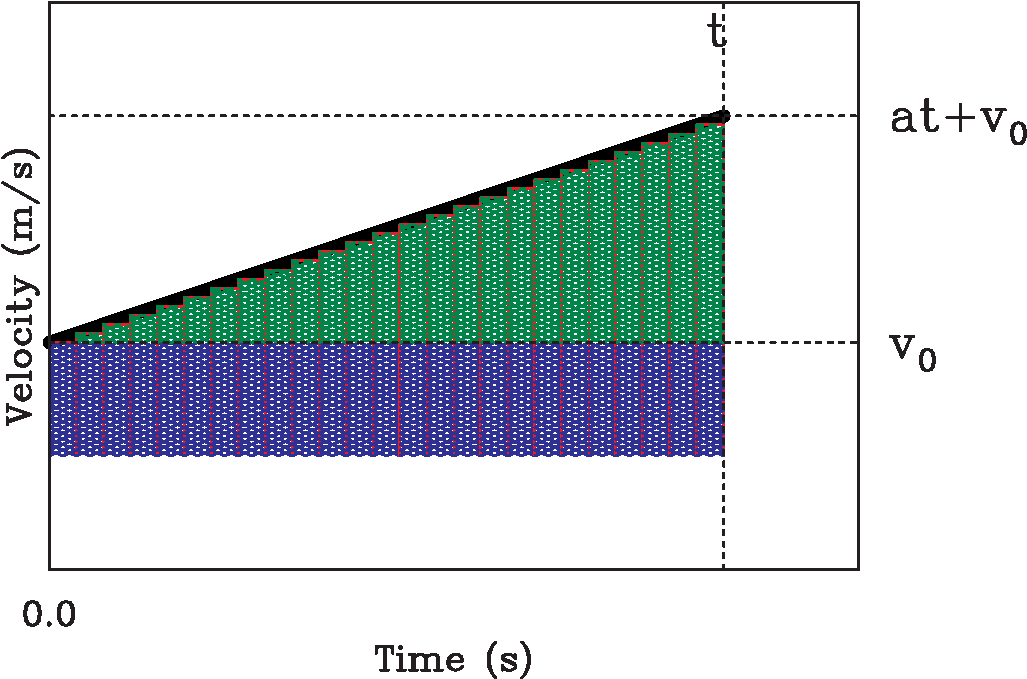
\includegraphics[width=0.6\textwidth]{area-under-v-full-crop.pdf}}

\bigskip

\pause
Area under blue part: $v_0 t$\\
Area under green part: $\frac{1}{2} at^2$\\
Total change in position: $x(t) - x_0 = \frac{1}{2}at^2 + v_0 t$

\bigskip
\bigskip
\centerline{\Large Thus, {\color{Red}$x(t) = \frac{1}{2}at^2 + v_0 t + x_0$.}}
}

\frame{\frametitle{\textbf{For those who are familiar with calculus:}}

\begin{align*}
a(t) &= \rm{const}.\\
v(t) &= \int a\,dt &=& at + C_1 \\
x(t) &= \int v\,dt = \int (at + C_1) dt &=& \frac{1}{2}at^2 + C_1 t + C_2
\end{align*}

\BS

A little thought reveals that $C_1$ is the initial velocity $v_0$ and $C_2$ is the initial position $x_0$.\\
This gives us the things we just derived, but much more easily:


{\color{Red}
\Large
\begin{align*}
v(t) &=& at + v_0 \\
x(t) &=& \frac{1}{2}at^2 + v_0 t + x_0
\end{align*}}
}

\frame{\frametitle{\textbf{Free fall revisited}}

\centerline{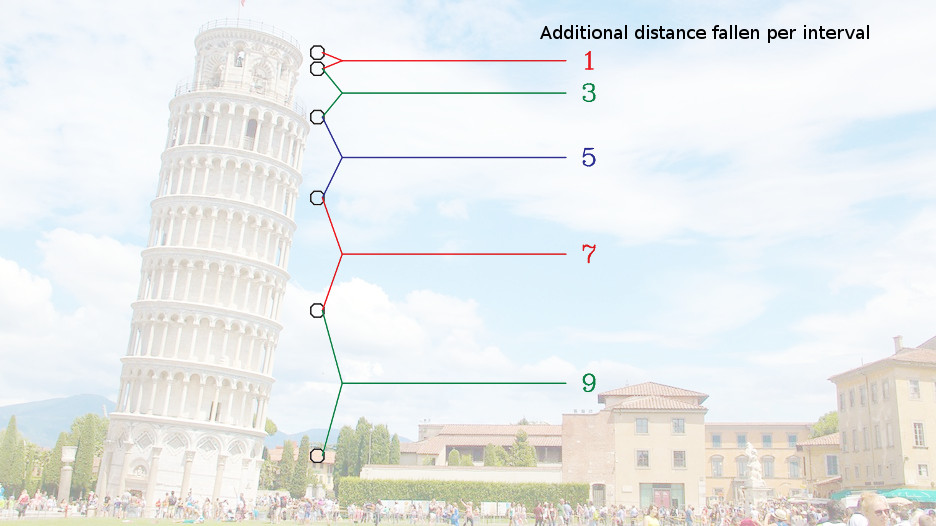
\includegraphics[width=0.9\textwidth]{pisa.jpg}}
\large\BS

\centerline{Adding these numbers together gives us 1, 4, 9, 16, 25...}
\centerline{The calculus above explains this: distance is proportional to {\it time squared!}}
}

\frame{\frametitle{\textbf{Coordinate systems}}
\Large
\BC
Position, velocity, and acceleration only make sense relative to a {\color{Red} coordinate system}.
\BS
{\it Any} coordinate system will get you the same answer, but you have to be {\it consistent}.
\EC
\large
\BS

In one dimension, like we're doing here, choosing a coordinate system means:

\BI
\item Choosing what position corresponds to $x=0$ (choosing an {\color{Red}origin})
\item Choosing which direction is positive and which is negative
\EI
}

\frame{\frametitle{\textbf{A warning for people who took high school physics!}}

\large
The value of the Earth's gravitational acceleration is ``$9.8\mss$ directed downward''. 

\BS

The constant $g$ simply refers to the {\it size} of this: $g \equiv 9.8\mss$.

\BS

Whether ``down'' is positive or negative depends on your choice of coordinate system. 

\BS

If you choose ``up'' to be positive, then you might write for a falling object ``$x(t)=-\frac{1}{2}gt^2$'', but $g$ 
itself {\it always represents a positive value}.
}

\end{document}
